%%%%%%%%%%%%%%%%%%%%%%%%%%%%%%%%%%%%%%%%%
% Structured General Purpose Assignment
% LaTeX Template
%
% This template has been downloaded from:
% http://www.latextemplates.com
%
% Original author:
% Ted Pavlic (http://www.tedpavlic.com)
%
% Note:
% The \lipsum[#] commands throughout this template generate dummy text
% to fill the template out. These commands should all be removed when 
% writing assignment content.
%
%%%%%%%%%%%%%%%%%%%%%%%%%%%%%%%%%%%%%%%%%

%----------------------------------------------------------------------------------------
%	PACKAGES AND OTHER DOCUMENT CONFIGURATIONS
%----------------------------------------------------------------------------------------

\documentclass[10pt]{report}
\usepackage{csquotes}
\usepackage{titlesec}

\usepackage{fancyhdr} % Required for custom headers
\usepackage{lastpage} % Required to determine the last page for the footer
\usepackage{extramarks} % Required for headers and footers
\usepackage{graphicx} % Required to insert images
\usepackage{multirow}
\usepackage{array}
\usepackage{lipsum} % Used for inserting dummy 'Lorem ipsum' text into the template
\usepackage{epstopdf} % to include eps graphics pdf
\usepackage{listings}
\usepackage{color}
\usepackage{caption}
\usepackage[a4paper,total={6in, 4in}]{geometry}
\usepackage{graphicx}
\usepackage{fancyhdr}
\usepackage[a4]{crop}
\usepackage{tikz}
\usepackage{float}
\usepackage{amsmath}
\usepackage{setspace}
\usetikzlibrary{calc}
\usepackage{subfig}
\usepackage{titlesec}
\usepackage{pdfpages}
%\newcommand{\sectionbreak}{\clearpage}
\topmargin=-0.45in
\evensidemargin=0in
\oddsidemargin=0in
\textwidth=6.5in
\textheight=9.5in
\headsep=.50in 
\footskip=.50in

\usepackage{chngcntr}
\counterwithin{figure}{chapter}

\linespread{1.5} % Line spacing
%\titleformat*{\section}{\LARGE\bfseries}
%\titleformat*{\subsection}{\Large\bfseries}
%\titleformat*{\subsubsection}{\Large\bfseries}
%\titleformat*{\paragraph}{\large\bfseries}
%\titleformat*{\subparagraph}{\large\bfseries}

% Set up the header and footer
\pagestyle{fancy}
%\nouppercase
\lhead{} % Top left header
\chead{} % Top center header
\rhead{\nouppercase{\leftmark}}  % Top right header
%{Real time pedestrian detection using CENTRIST feature with distance estimation
\lfoot{Dept of Electronics, Model Engineering College} % Bottom left footer
\cfoot{} % Bottom center footer
\rfoot{\thepage} % Bottom right footer
\renewcommand\headrulewidth{0.4pt} % Size of the header rule
\renewcommand\footrulewidth{0.4pt} % Size of the footer rule

\setlength\parindent{0pt} % Removes all indentation from paragraphs

%----------------------------------------------------------------------------------------
%	TITLE PAGE
%----------------------------------------------------------------------------------------
\tolerance=1
\emergencystretch=\maxdimen
\hyphenpenalty=10000
\hbadness=10000

\begin{document}




\begin{titlepage}
%\AddToShipoutPictureBG*{
\includegraphics[width=\paperwidth,height=\paperheight]{seminar.png}};
%\ClearshipoutPicture
\pagestyle{empty}
\begin{tikzpicture}[overlay,remember picture]
\draw [line width=3pt,rounded corners=1pt,]
    ($ (current page.north west) + (1cm,-1cm) $)
    rectangle
    ($ (current page.south east) + (-1cm,1cm) $);       
\end{tikzpicture}
\newcommand{\HRule}{\rule{\linewidth}{0.5mm}} % Defines a new command for the horizontal lines, change thickness here

\center % Center everything on the page
 
%----------------------------------------------------------------------------------------
%	HEADING SECTIONS
%----------------------------------------------------------------------------------------
\linespread{1.0}
%% \HRule \\[0.1cm]
    {\Huge \bfseries DESIGN AND IMPLEMENTATION OF CFAR IN SONAR BEAMFORMING  \par}

\vspace{1.1cm}
   % \HRule \\[1.5cm]
%{ \huge \bfseries  REAL TIME PEDESTRIAN DETECTION USING CENTRIST FEATURE WITH DISTANCE MEASURE } \\[0.5cm] % Title of your Presentation
%\\[0.5cm]


%----------------------------------------------------------------------------------------
%	LOGO SECTION
%----------------------------------------------------------------------------------------


\includegraphics[scale=.75]{mec.png}\\ % Include a department/university logo - this will require the graphicx package
 

%----------------------------------------------------------------------------------------
%	AUTHOR SECTION
%----------------------------------------------------------------------------------------

% If you don't want a supervisor, uncomment the two lines below and remove the section above
\Large \emph{BY,}\\

NPOL - GROUP4\\[0.5CM]
\centering
Alwin Thampi\\
\centering
Anagha C H\\
\centering
Finny Philip Biju\\
\centering
Jibin Joseph Rocha\\ \\
\centering
Anusree M\\[1.5cm]


%-------------------------------------------------------------------------------------------
\large \emph{Department of Electronics Engineering, \\
Model Engineering College, \\ Thrikkakara,
Kochi-682021,\\  Kerala.}
\\[0.5cm] % Minor heading such as course title

\Large \emph{OCTOBER 2021}
%----------------------------------------------------------------------------------------

\vfill % Fill the rest of the page with whitespace

\end{titlepage}






%----------------------------------------------------------------------------------------
%	TABLE OF CONTENTS
%----------------------------------------------------------------------------------------




\newpage


\clearpage
%\setcounter{page}{1}
%----------------------------------------------------------------------------------------
%	TABLE OF CONTENTS
%----------------------------------------------------------------------------------------

%\setcounter{tocdepth}{1} % Uncomment this line if you don't want subsections listed in the ToC
\pagenumbering{roman}

\fontsize{12}{12}\selectfont 
\newpage
\thispagestyle{empty}
 
\thispagestyle{empty}
\tableofcontents
%\newpage
\thispagestyle{empty}
\listoffigures
\addcontentsline{toc}{chapter}{\numberline{}LIST OF FIGURES} 
 % \addcontentsline{toc}{chapter}{\numberline{}LIST OF FIGURES}

 \newpage

\clearpage
%\pagenumbering{arabic}
\setcounter{page}{1}
\setstretch{1.3}



\chapter {INTRODUCTION}
\label{intro}
\pagenumbering{arabic}

\setlength{\parindent}{10ex}
The primary task of SONAR used in submarines is to detect all objects within the area 
of observation and to estimate their positional coordinates. Constant false alarm rate (CFAR) processors alleviate the problems of 
automatic target detection when the interference power is unknown or time varying. The goal 
of a CFAR processor is to maintain a constant false alarm probability, while maximizing the 
detection probability. It does so by estimating the interference power in the resolution cell 
under examination. A target is declared to be present if the power in the cell under test exceeds 
some fixed multiple of the estimated interference power.










The CFAR detector contains four main elements namely: Cell Under Test (CUT), 
Guard cells, Reference cells & CFAR multiplier. The threshold level setting of the CFAR 
detector should follow the background noise power that is estimated by an algorithm depends 
on the detection environments. Targets should be detected in different detection environments. 
These environments are homogeneous environment (single target or multi-targets) and nonhomogeneous environment (closed multi-targets or clutter edge). Corresponding to these 
environments various CFAR detector had been developed, namely, Cell Averaging CFAR 
(CA-CFAR), Greatest Of (GO-CFAR), Smallest Of (SO-CFAR), Ordered Statistic (OSCFAR). Modem radar systems support automatic detection modes in which some function of 
the envelope detector output at a range-Doppler resolution cell is compared with a threshold 
number, T. If the threshold is exceeded, then a target is declared to be present

\chapter {LITERATURE REVIEW}

The paper “Radar Target detection using Cell Evaluation Method for Industrial Safety” 
by Sambath p et.al gives an idea about the normal cfar architecture. It mentions about the main 
elements of the cfar detector. They are Cell Under Test (CUT), Guard cells, Reference cells 
and CFAR multiplier. The Cell Under Test (CUT) is where the threshold is to be applied based 
on which the target is declared present or not. Potential objects in CUTs are found from 
identifying the local maxima’s which is scale dependent and not very well defined. The guard 
cells are used to estimate the threshold in CUT precisely. The samples contained in the guard 
cells are not use for any calculation. This is done mainly to eliminate any spill over of the target 
in the CUT if there is any extended target present that could mess up with the calculation of 
the threshold. This helps in better estimation of the noise level. The samples reference cells are 
used for the estimation of the noise level thereby helps in calculating the threshold. The more 
the number of reference cells chosen, the better estimation of threshold is achieved.

 
 
 
 \begin{figure}[h]
 	\centering
 	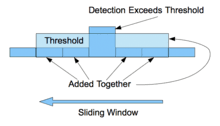
\includegraphics[scale = 1]{download.png}
 	\caption{Typical CA CFAR Architecture}
 \end{figure}



\end{figure}



The paper “Radar CFAR Thresholding in Clutter and Multiple Target Situations” by 
Hermann Rohling et.al gives an idea about the cfar detection process. It discusses how the 
threshold value is calculated in existing cfar systems using the sliding window technique. The 
data available in the reference window enter into an algorithm for the calculation of the decision 
threshold. A CFAR method is discussed using as the CFAR threshold one single value selected 
from the so-called ordered statistic. This procedure has some advantages over cell averaging 
CFAR, especially in cases where more than one target is present within the reference window 
on which estimation of the local clutter situation is based, or where this reference window is 
crossing clutter edges.



The paper “Design and Implementation of a New CFAR Based on Weighted and 
Statistical Algorithms” by Gufran M. Hatem et.al gives an idea about the different CFAR 
algorithms. The CFAR, which can work with the most environment (homogeneous and nonhomogeneous) and most of the target situations (single target, multiple targets, closely spaced 
multiple targets etc.), has been discussed. The threshold level setting of the CFAR detector 
should follow the background noise power that is estimated by an algorithm depends on the 
detection environments. Targets should be detected in different detection environments. These 
environments are homogeneous environment (single target or multi-targets) and nonhomogeneous environment (closed multi-targets or clutter edge). Corresponding to these 
environments various CFAR detector had been developed, namely, Cell Averaging CFAR 
(CA-CFAR), Greatest Of (GO-CFAR), Smallest Of (SO-CFAR), Ordered Statistic (OSCFAR).


\chapter {DESIGN}
\section{CFAR Architecture}
The Constant false alarm rate (CFAR) is a basic detection algorithm applied on the 
received signal of the SONAR. This algorithm determines a fixed threshold based on the 
background noise. If any sample exceeds the estimated threshold level, it is declared as the 
target is present else it is declared as the target is not present.

The CFAR detector contains four main elements namely:


\begin{itemize}
   \vspace{0.4cm}
   \item Cell Under Test(CUT)
   \vspace{0.4cm}
   \item Guard Cells
   \vspace{0.4cm}
   \item Reference cells
   \vspace{0.4cm}
   \item CFAR Multiplier 
 \end{itemize}
  \begin{figure}[h]
 	\centering
 	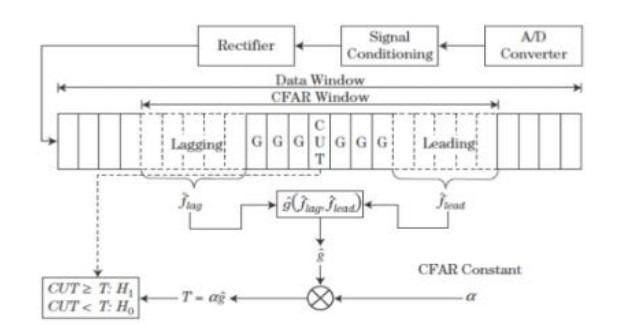
\includegraphics[scale=1]{c.jpg}
 	\caption{Typical CA CFAR Architecture}
 \end{figure}

 
 
\newpage 
Figure shows a simple CFAR detector. Once the threshold over all the CUT in the range 
is calculated, it is multiplied with the CFAR constant α and compared with the CUT. If the 
samples in the CUT is greater than or less than the estimated threshold H0 or H1 is chosen 
accordingly. In this project, Cell Averaging CFAR is discussed
\section{CA CFAR Block Diagram}
The CA-CFAR processor block diagram is shown in Figure. For the linear operations, 
it is required to add all values stored in the reference cells registers of the leading/lagging 
windows for computing the average. In order to perform this operation, it is not necessary to 
add all values each time that one value from the reference cells registers is inserted and deleted.
  \begin{figure}[h]
 	\centering
 	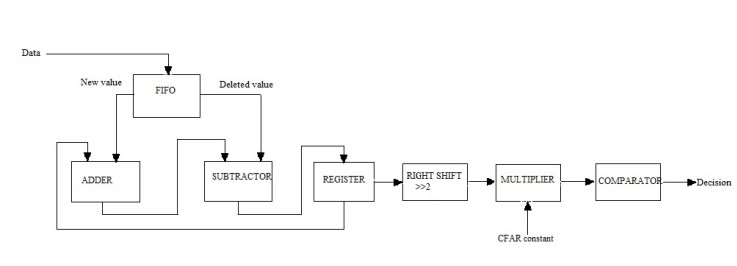
\includegraphics[scale=1]{cfar.jpg}
 	\caption{Typical CA CFAR Architecture}
 \end{figure}



\end{figure}
Once a value is inserted and other one deleted, the preceding result can be used to compute the 
next result without adding all values. Only by adding and subtracting the newest and oldest 
values respectively, the next result is obtained. This whole operation can be performed by an 
accumulator, which computes the average of values on each window. The accumulator consists 
of an adder, which receives the incoming value, a subtracter, which selects the oldest value 
stored in the reference cells of leading/lagging window, a register to store the accumulated 
value. A left shifter that performs the division is needed to compute the average value. Because 
of the left shifter, the number of reference cells must be a power of two. After calculating the 
average, it is given to the multiplier block which multiplies this value with CFAR constant, 
followed by a comparator block which compares the threshold value with the value in CUT.
\section{OS CFAR}
Cell‐averaging CFAR was the first of the CFAR methods. Assuming homogene‐
ous Gaussian white noise, through a sliding window, CA‐CFAR estimates the noise level
of the cell under test, CUT, through an arithmetic sum of N adjacent cells . In heteroge‐
neous environments, however, CA‐CFAR performance rapidly degrades.
Ordered Statistics CFAR, OS‐CFAR, had been developed to compensate for
much of CA‐CFAR’s pitfalls. Rather than taking the arithmetic mean of adjacent cells,
OS‐CFAR ranks the N adjacent cells from smallest to largest and multiplies the k
th larg‐
est cell to the appropriate threshold multiplier to set the threshold level.
\begin{figure}[h]
	\centering
	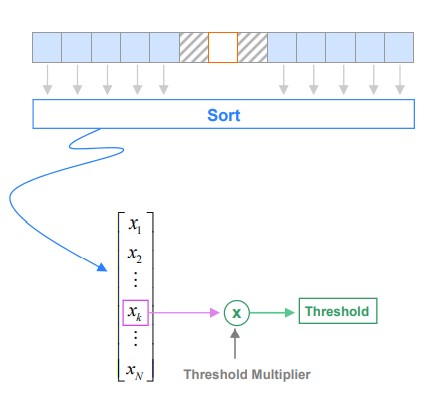
\includegraphics[scale=1]{os.jpg}
	\caption{OS CFAR Architecture}
\end{figure}
The kth‐ranked cell could be the median ranked value or even the largest value. As simulations will show, the larger x(k), the smaller the CFAR‐loss in homogeneous environment but the less the resistance to target masking and clutter‐edge transition
 
\chapter {Tools Analysis}
\section{Sofware Requirements}
\subsection{Matlab}
MATLAB allows matrix manipulations, plotting of functions and data, implementation 
of algorithms, creation of user interfaces, and interfacing with programs written in other 
languages. MATLAB lets you take your ideas from research to production by deploying to 
enterprise applications and embedded devices, as well as integrating with Simulink and ModelBased Design. Simulink is a block diagram environment for multi domain simulation and 
Model-Based Design. It supports system-level design, simulation, automatic code generation, 
and continuous test and verification of embedded systems
\subsection{Xilinx System Generator}
The Xilinx System Generator for DSP is a plug-in to Simulink that enables designers 
to develop high-performance DSP systems for Xilinx FPGAs. Designers can design and 
simulate a system using MATLAB, Simulink, and Xilinx library of bit/cycle-true models. The 
tool will then automatically generate synthesizable Hardware Description Language (HDL) 
code mapped to Xilinx pre-optimized algorithms.
\subsection{Xilinx Vivado}
The Vivado High-Level Synthesis compiler enables C, C++ and SystemC programs to 
be directly targeted into Xilinx devices without the need to manually create RTL. The Vivado 
IP Integrator allows engineers to quickly integrate and configure IP from the large Xilinx IP 
library. The Integrator is also tuned for MathWorks Simulink designs built with Xilinx’s 
System Generator and Vivado High-Level Synthesis.
\section{Hardware Requirements}
\subsection{Xilinx Kintex Ultrascale FPGA}
Kintex® UltraScale™ devices provide the best price/performance/watt at 20nm and include the highest signal processing bandwidth in a mid-range device, next- generation transceivers. The family is ideal for packet processing in 100G networking and data center applications as well as DSP-intensive processing needed in next- generation medical imaging, 8k4k video, and heterogeneous wireless infrastructure.

 \chapter {Simulation Results}
\section{Matlab}


 \begin{figure}[h]
	\centering
	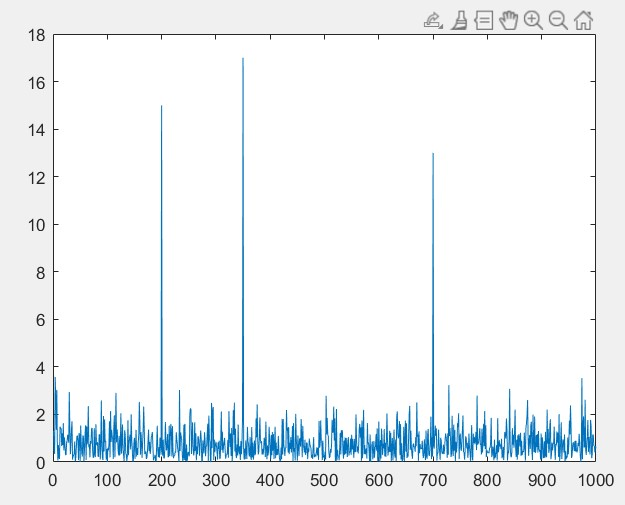
\includegraphics[scale=1]{sim.jpg}
	\caption{Noise Generation (Noise + Target)}
\end{figure}

\newpage
\subsection{Detection}
 \begin{figure}[h]
	\centering
	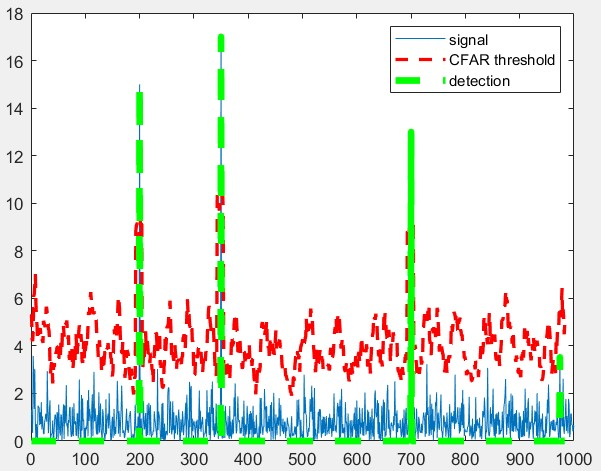
\includegraphics{sim2.jpg}
	\caption{Detection using CA CFAR}
\end{figure}
\newpage\section{Vivado}
 \begin{figure}[h]
	\centering
	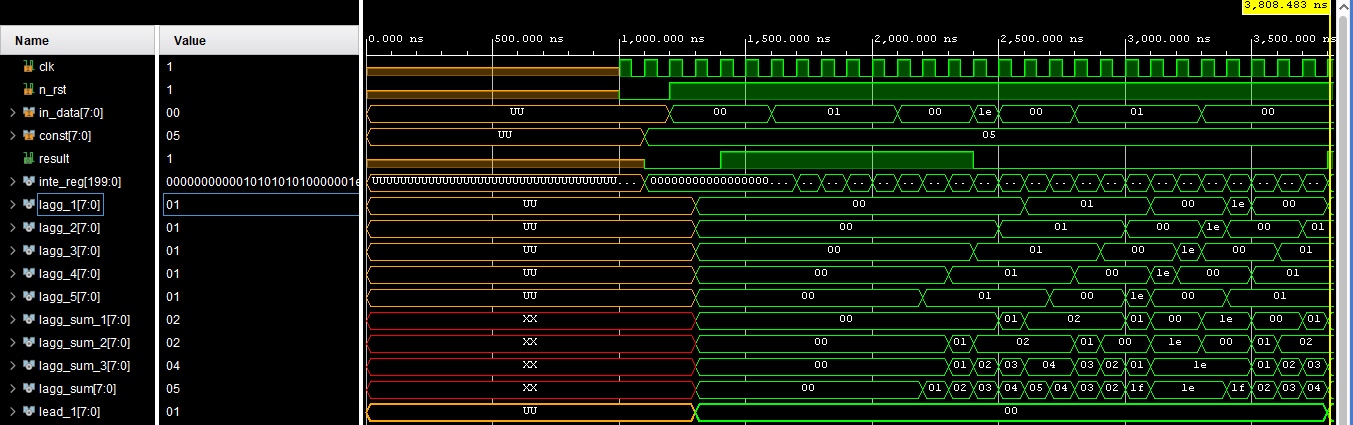
\includegraphics[width=180mm,scale=2]{final1.png}
	\caption{Vivado simulation result}
\end{figure}
\begin{figure}[h]
	\centering
	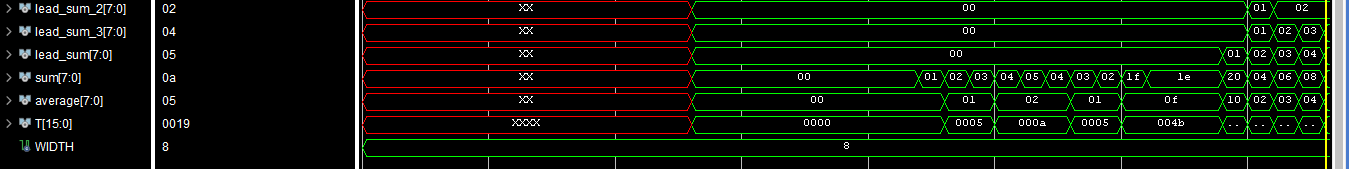
\includegraphics[width=180mm,scale=2]{final2.png}
	\caption{Vivado simulation result}
\end{figure}









\end{chapter}
\newpage
\begin{thebibliography}{999}
\addcontentsline{toc}{chapter}{REFERENCES}
\item {  Abu & Diamant, R. (2020). CFAR detection algorithm for objects in sonar images. IET Radar, Sonar & Navigation, 14(11), 1757-1766.
\vskip 0.25cm
\item  {Rohling, H. (1983). Radar CFAR thresholding in clutter and multiple target situations. IEEE        transactions on aerospace and electronic systems, (4), 608-621.
\vskip 0.25cm
\item {Saeed, T., Hatem, G., Sadah, J. A., & Ziboon, H. (2020). Design and Implementation of a New CFAR Based on Weighted and Statistical Algorithms.
\vskip 0.25cm
\item {Sambath, P. (2020). Radar Target detection using Cell Evaluation Method for Industrial Safety.
\vskip 0.25cm
\item {Kalyan, B., & Balasuriya, A. (2004, April). Sonar based automatic target detection scheme for underwater environments using CFAR techniques: a comparative study. In Proceedings of the 2004 International Symposium on Underwater Technology (IEEE Cat. No. 04EX869) (pp. 33-37). IEEE


\end{frame}

\end{document}







